\section{Hello World}

对于大部分编程语言来说,第一个程序一般都是 ``Hello, World!''。

我们学习 \Deno 自然也不能免俗,
\Deno 主要支持 \TypeScript,所以对应代码如下:

\begin{table}[H]
    \begin{minted}{typescript}
console.log("Hello, World!");
    \end{minted}
    \caption{Hello World 程序}
    \label{code:beginner:hello-world}
\end{table}

对于 \Deno 而言,你还可以直接执行网络代码,所以同样的,可以使用:

\begin{table}[H]
    \begin{minted}{shell}
deno run "https://examples.deno.land/hello-world.ts"
    \end{minted}
    \caption{执行在线代码}
    \label{code:beginner:execute-online}
\end{table}

输出效果都是如下:

\begin{figure}[H]
    \centering
    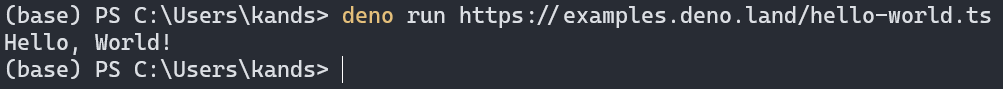
\includegraphics[scale=0.48]{pics/beginner-hello-world-p01.png}
    \caption{代码执行效果}
    \label{fig:beginner:hello-world:p01}
\end{figure}
